\documentclass[12pt, a4paper]{article}

\usepackage[margin=2.5cm]{geometry}
\usepackage{graphicx}
\usepackage{booktabs}
\usepackage{amsmath}
\usepackage{parskip}
\usepackage{float}

\begin{document}

% ── Title ──────────────────────────────────────────────────
\begin{center}
    {\LARGE \textbf{MLX 2.0 Regression Challenge}}\\[0.3cm]
    {\large CS3111 - Introduction to Machine Learning}\\[0.2cm]
    {\large Lab 02 Regression Report}\\[0.2cm]
    N.G.T.S.Gamage (UOM\_230194C) 
\end{center}

\hrule
\vspace{0.5cm}

% ── Approach 1 ─────────────────────────────────────────────
\section*{Approach 1: Random Forest}

Random Forest builds many decision trees independently using random subsets of the data. The final prediction is the average of all tree predictions. This technique, called \textit{bagging}, reduces variance and helps prevent overfitting compared to a single decision tree.

\begin{equation}
    \hat{y} = \frac{1}{T} \sum_{t=1}^{T} f_t(x)
\end{equation}

\textbf{Why chosen:} Random Forest was chosen as the first approach because it is robust to noisy data and missing values, requires minimal hyperparameter tuning, and handles both numerical and categorical features well, making it a reliable baseline for a real-world dataset like this one.


\textbf{Drawbacks:} 
\begin{itemize}
    \item High memory usage when using many trees
    \item Slower prediction time compared to simpler models
    \item Less interpretable than a single decision tree
    \item May underperform when features have complex sequential dependencies
\end{itemize}

% ── Approach 2 ─────────────────────────────────────────────
\section*{Approach 2: XGBoost}

XGBoost builds trees \textit{sequentially}, where each new tree learns from the mistakes of the previous ones. This is called \textit{gradient boosting}:. It also has built-in regularisation to reduce overfitting. The learning rate controlling how much each new tree contributes to the final model.

\textbf{Why chosen:} XGBoost was chosen as the second approach because it often achieves higher accuracy than Random Forest by learning from mistakes iteratively. It also includes built-in regularisation (L1 and L2) to control overfitting, making it well-suited for complex datasets.

\textbf{Drawbacks:} 
\begin{itemize}
    \item More sensitive to hyperparameter choices — requires careful tuning
    \item Slower to train when the number of estimators is large
    \item More prone to overfitting if the learning rate is set too high
    \item Harder to interpret compared to simpler models
\end{itemize}

% ── Evaluation Metrics ─────────────────────────────────────
\section*{Evaluation Metrics}

Three metrics were used to evaluate both models on a local validation set (20\% of training data):

\textbf{RMSE} (Root Mean Squared Error) — measures the average prediction error. Large errors are penalised more heavily because errors are squared. \textit{Lower is better.}

\begin{equation*}
    \text{RMSE} = \sqrt{\frac{1}{n} \sum_{i=1}^{n} (y_{\text{true}} - y_{\text{pred}})^2}
\end{equation*}

\textbf{MAE} (Mean Absolute Error) — measures the average absolute difference between predicted and actual values. Treats all errors equally. \textit{Lower is better.}

\begin{equation*}
    \text{MAE} = \frac{1}{n} \sum_{i=1}^{n} |y_{\text{true}} - y_{\text{pred}}|
\end{equation*}

\textbf{R\textsuperscript{2} Score} — measures how much of the variation in popularity scores the model explains. A score of 1.0 is perfect; 0 means the model is no better than predicting the average. \textit{Higher is better.}

\begin{equation*}
    R^2 = 1 - \frac{\sum(y_{\text{true}} - y_{\text{pred}})^2}{\sum(y_{\text{true}} - \bar{y})^2}
\end{equation*}

% ── Results ────────────────────────────────────────────────
\section*{Results and Comparison}

\begin{table}[H]
    \centering
    \begin{tabular}{lccc}
        \toprule
        \textbf{Model} & \textbf{RMSE} $\downarrow$ & \textbf{MAE} $\downarrow$ & \textbf{R\textsuperscript{2}} $\uparrow$ \\
        \midrule
        Random Forest & 11.3068 & 6.6698 & 0.7255 \\
        XGBoost       & 12.8336 & 9.0323 & 0.6464 \\
        \bottomrule
    \end{tabular}
    \caption{Local validation results}
\end{table}

\begin{table}[H]
    \centering
    \begin{tabular}{lcc}
        \toprule
        \textbf{Model} & \textbf{Kaggle Public RMSE} & \textbf{Kaggle Private RMSE} \\
        \midrule
        Random Forest & 10.8188 & 10.7959 \\
        XGBoost       & 12.5064 & 12.5300 \\
        \bottomrule
    \end{tabular}
    \caption{Kaggle leaderboard scores}
\end{table}

\textbf{Discussion:} Random Forest performed better than XGBoost across all metrics. Its RMSE of 10.82 on Kaggle means predictions were on average about 10.8 popularity points away from the true score. The R\textsuperscript{2} of 0.7255 shows it explained 72.5\% of the variation in song popularity, which is a solid result for a real-world dataset.

XGBoost scored higher RMSE (12.51) and lower R\textsuperscript{2} (0.6464), meaning it captured less of the underlying patterns. This is likely because XGBoost requires careful hyperparameter tuning to reach its best performance, which was not done here. With proper tuning, XGBoost would likely match or outperform Random Forest.

Both models generalised well. Their Kaggle scores were slightly better than their local validation scores, confirming no overfitting occurred.

% ── Screenshots ────────────────────────────────────────────
\section*{Kaggle Submission Screenshots}

\begin{figure}[H]
    \centering
    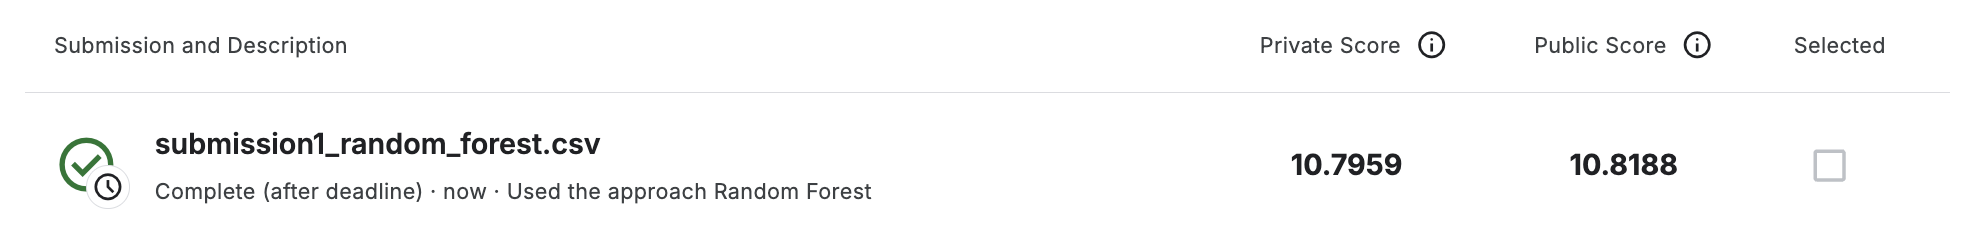
\includegraphics[width=\textwidth]{screenshot_rf.png}
    \caption{Kaggle submission — Random Forest (Public RMSE: 10.8188, Private RMSE: 10.7959)}
\end{figure}

\begin{figure}[H]
    \centering
    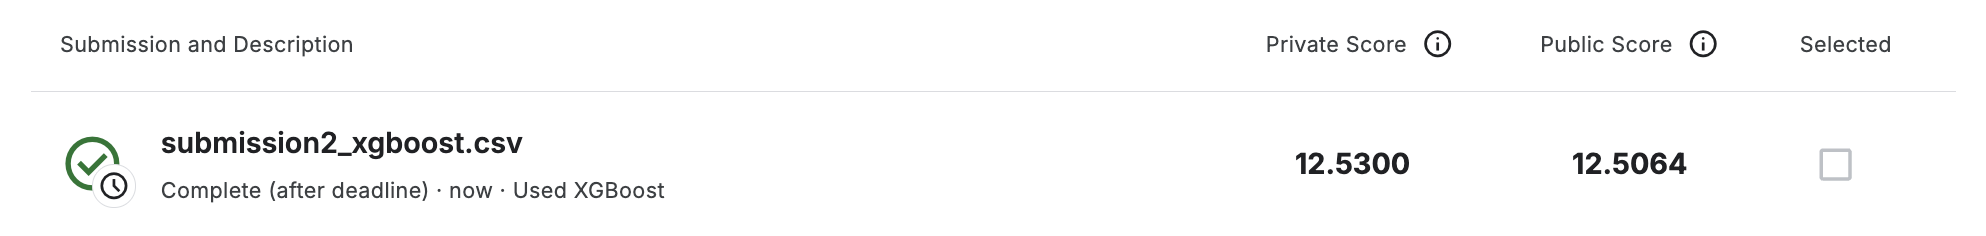
\includegraphics[width=\textwidth]{screenshot_xgb.png}
    \caption{Kaggle submission — XGBoost (Public RMSE: 12.5064, Private RMSE: 12.5300)}
\end{figure}

\end{document}